%% The following is a directive for TeXShop to indicate the main file
%%!TEX root = diss.tex

\chapter{Luminescence from Organic Molecules}
\label{ch:opv}

Prior to the work done in this thesis, \ac{STML} from a single organic molecule has not yet been detected on our system. To optimize and ensure the viability of the experimental setup, \ac{STML} was performed on prototypical organic semiconducting molecules \ac{PTCDA} \citep{Rzeznicka2011, Kimura2019} and \ac{ZnPc} \citep{Zhang2016, Doppagne2017, Zhang2017, Imada2016, Doppagne2018, Miwa2019}, both of which have had successful reports of \ac{STML} experiments. Fluorination of phthalocyanine molecules have previously been demonstrated as a method to tune the electronic and optical energies of the molecule in bulk \citep{schwarze2016band, warren2019controlling}. Further experiments were carried out on \ch{F8ZnPc} to explore the effects of fluorination on the structural, electronic and optical properties of ZnPc.

During \ac{STML} experiments, the tip was parked on top of the molecule with a certain bias, and setpoint current. The shutter to the spectrometer was then opened for a certain exposure time $t_x$. The parameters for each \ac{STML} experiment will be listed as $V_b/I_t/t_x$.


\section{Plasmon emission from substrates}

Plasmon emission from the bare metallic surface can vary in energy and intensity depending on the geometry of the tip. Aside from attaining a sharp metallic tip for \ac{STM} and \ac{STS}, the tip needs to be poked and pulsed until it produce a strong plasmonic response in the energy region of interest. Representative spectra of the plasmon on Ag(111) and Au(111) with Ag tip is presented in \autoref{fig:opv:metal-plasmon}. The same Ag tip was used to acquire both spectra, allowing for comparison. The plasmon emission on the Au(111) is weaker in intensity and lower in energy than the emission on Ag(111). The lower intensity was likely because of the change in tip-sample position due to the lower height of the thin film, resulting in a drop of about an order of magnitude in intensity. The shift in photon energy was caused by the inherent dielectric response of the materials \citep{olmon2012optical, yang2015optical}.

% The shift in photon energy was because of the dielectric function of the two materials: gold with a minimal imaginary dielectric function at \SI{1.8}{eV} or \SI{680}{nm} \citep{olmon2012optical}, and silver at \SI{3.2}{eV} or \SI{390}{nm} \cite{yang2015optical}.

\begin{figure} [h]
    \centering
    %\includegraphics[width=3in]{file}
    \caption{\FIXME{Ag and Au plasmons, spectra taken with the same tip.}}
    \label{fig:opv:metal-plasmon}
\end{figure}



When \ac{STML} experiments are carried out on molecular species, they are decoupled by a bilayer (2\ac{ML}) NaCl, which can modify the plasmon emission. Using the same Ag tip, modification of the plasmon emission on Ag(111) and Au(111) by layers of NaCl can be seen in \autoref{fig:opv:nacl-plasmon}. Overall, there is an enhancement and redshift in the detected photons when compared to the bare metal substrate.


\begin{figure} [h]
    \centering
    %\includegraphics[width=3in]{file}
    \caption{\FIXME{Ag and Au plasmons, modified by nacl (2ML and 3ML?)}}
    \label{fig:opv:nacl-plasmon}
\end{figure}

Thicker layers of NaCl further dissociate the molecule from the metallic substrate, allowing for a more accurate study of the intrinsic properties of the molecule \citep{repp2005molecules}. Thicker layers of NaCl have demonstrated enhanced molecular luminescence; the effect of a smaller tip-sample junction and more effective dissociation of the molecule from the metal \citep{Zhang2017,Kroger2018}. However, a closer tip results in stronger interactions between the tip and the molecule, affecting the stability of the molecule on the NaCl. Bilayer NaCl gave the most consistent and stable configurations for \ac{STML}.



\section{Study of {ZnPc}}

\ac{ZnPc} is a relatively planar organic semiconducting molecule that can be thermally deposited, making it optimal for \ac{SPM} study. Because of previous reports of \ac{STML} on ZnPc, this molecule was used to test the \ac{STML} capabilities of our system. 

% The structure of the ZnPc is shown in \autoref{fig:opv:znpc-stm}. The substrate was (2ML)NaCl/Au(111) thin film, and the tip used was the Pt/Ir tip dipped in gold. At biases higher than \SI{1}{V}, the ZnPc molecule rotates to give a 16-lobed structure. The non-rotating molecule has an 8-lobed structure, which could be seen if the molecules were ``anchored" by some defect or step edge, or was dimerized to another molecule.  

% \begin{figure} [h]
%     \centering
%     %\includegraphics[width=3in]{file}
%     \caption{\FIXME{Show stm of ZnPc (-1V, 1.0, 2.0), also with dimerize }}
%     \label{fig:opv:znpc-stm}
% \end{figure}

% The electronic structure was then probed using \ac{STS}. The \ac{LDOS} along with the molecular orbitals at the resonances are shown in \autoref{fig:opv:znpc-sts}.

% \begin{figure} [h]
%     \centering
%     %\includegraphics[width=3in]{file}
%     \caption{\FIXME{Show sts of ZnPc on Au(111)}}
%     \label{fig:opv:znpc-sts}
% \end{figure}

% Previous reports of ZnPc on this substrate show that the electronic states of the molecule do not change much in structure, and only experience a rigid shift of $\approx \SI{-1}{eV}$ in energy when compared to (2ML)NaCl/Au(111), due to the lower work function of (2ML)NaCl/Ag(111) \citep{Doppagne2017,Doppagne2018}. With an optimized Ag tip, photoluminescence was detected on the molecule, with an emission peak at \SI{630}{nm} or \SI{1.96}{eV} (\autoref{fig:opv:znpc-stml}).

To maximize \ac{STML} signal, ZnPc was deposited on (2ML)NaCl/Ag(111) and probed with the Ag tip. With parameters $\SI{3.0}{V}/\SI{300}{pA}/\SI{300}{s}$, we were able to detect emission from ZnPc at \SI{630}{nm} or \SI{1.96}{eV} (\autoref{fig:opv:znpc-stml}).

\begin{figure} [h]
    \centering
    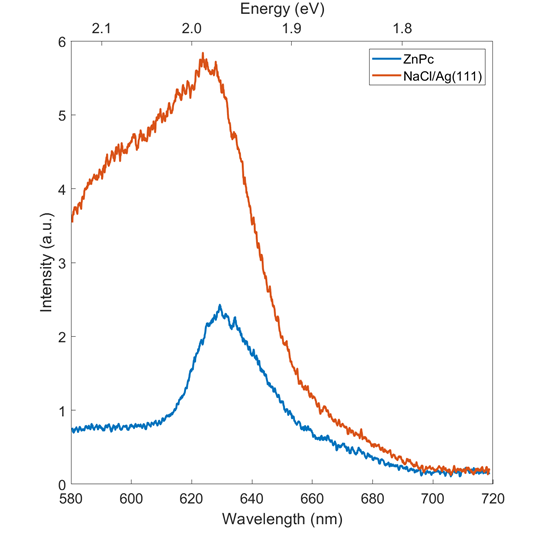
\includegraphics[width=3in]{pictures/stml_znpc_ag111.png}
    \caption{\FIXME{show inset with the molecule on surface, and position of tip on molecule}}
    \label{fig:opv:znpc-stml}
\end{figure}



\subsection{Discussion}

Previous reports of \ac{STML} on ZnPc and PTCDA are summarized in 

Energy of tunnelling induced photon emission from ZnPc have a reported a peak at \SI{1.9}{eV}, at bias \SI{-2.5}{V} \citep{Zhang2016,Zhang2017,Doppagne2017,Doppagne2018}. 

There are two distinctions between the detected data in \autoref{fig:opv:znpc-stml} and previously reported data: the energy of the exciton optical gap in our data is \SI{0.06}{eV} higher, and the emission peak is significantly broader. Previously reported data have peak \ac{FWHM} of approximately \SI{15}{meV}, while our emission peak has \ac{FWHM} \SI{63}{meV}, about 4 times broader.

Previous reports of \ac{STS} on this system report that the \ac{HOMO} and \ac{LUMO} are located at \SI{-2.3}{eV} and \SI{0.9}{eV}, respectively \citep{Doppagne2017}.




\section{Study of {PTCDA}}

The next system studied was the \ac{PTCDA} molecule on (2ML)NaCl/Au(111). As discussed before, the Au(111) thin film sample is slightly out of focus of the lens, resulting in weaker signals. However, \ac{PTCDA} is highly electronegative, and the (2ML)NaCl/Ag(111) substrate has a low work function, resulting in a charged PTCDA \citep{cochrane2017single,cochrane2018molecularly}. By using Au(111), which has a higher work function, as the metallic substrate, the PTCDA molecule was not charged on the surface, giving a simpler system to probe. Additionally, previous preliminary work in our group has demonstrated luminescence quenching on the PTCDA/(2ML)NaCl/Ag(111) system \citep{roussy2016coupling}, although a recent publication has shown otherwise \citep{Kimura2019}.

Photoluminescence from a single PTCDA on (2ML)NaCl/Au(111) was detected, with an emission peak at \SI{670}{nm} or \SI{1.85}{eV}, at \SI{3}{V}/\SI{200}{pA}/\SI{300}{s}.


\begin{figure} [h]
    \centering
    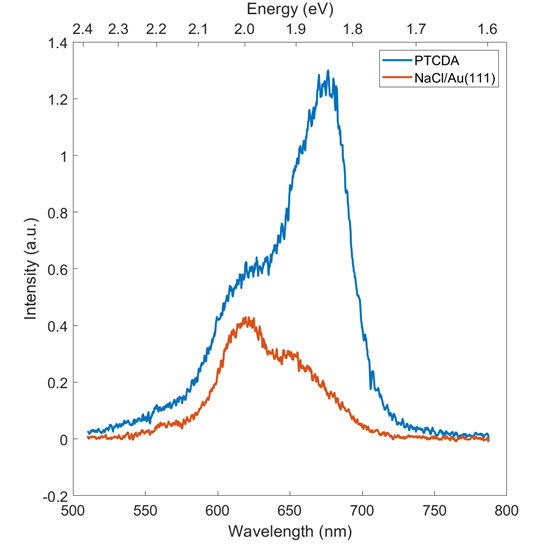
\includegraphics[width=3in]{pictures/stml_ptcda_au111.png}
    \caption{\FIXME{show inset with the molecule on surface, and position of tip on molecule}}
    \label{fig:opv:ptcda-stml}
\end{figure}





\subsection{Discussion}

A recent work by \emph{Kimura et al.} was the first report of single molecule \ac{STML} on a negatively charged PTCDA, with a substrate of (3ML)NaCl/Ag(111). The authors corresponded the $S$ \FIXME{notation for the franck condon transitions} transition to an emission peak at \SI{2.45}{eV} with bias onset at $V_b=\SI{-2.2}{V}$ \citep{Kimura2019}. The energy of the emission peak seen in \autoref{fig:opv:ptcda-stml} does not correspond to the previously reported result. 

Additionally, our detected emission is broadened, with a \ac{FWHM} of \SI{100}{meV}. The broadness and energy is similar to the \ac{CT} emission seen on the bilayer system, however, there were no neighbouring molecules in our system to broaden the signal or to form a \ac{CT} state. 

An earlier study looked at \ac{STML} on a bilayer of \ac{PTCDA}, with the first monolayer acting as the decoupling layer. The authors found a broad \ac{CT} emission at \SI{1.75}{eV} for $V_b =\SI{2.5}{V}$, and an additional weaker $S_{10}$ transition at \SI{2.35}{eV} for $V_b = \SI{3.0}{V}$ \citep{Rzeznicka2011}. 

A possible explanation for our spectra in \autoref{fig:opv:ptcda-stml} is the tunnelling






\section{Study of \ch{F8ZnPc}}






\subsection{Effects of adsorption geometry}





%%%%%
